\section{Wireless Data Transfer}
This section describes the most important point for the research. If the data is not transferred wireless to the external system blablabla

\subsection{Original idea}
EtherCAT is already used on the exoskeleton as stated in section \ref{sec:etherCat}. This lead to the first point, whether the current EtherCAT-configuration could be extended. The exoskeleton (E) and the receiver (R) would both be running Simulink. The receiver would then process the data and send it to the interface (I). This leaves the possibility to  extend to multiple interfaces, by putting a broadcaster (B) between the receiver and the interface(s). A visual representation of this model can be found in figure \ref{fig:catmodel}. However, the EtherCAT-blocks in Matlab \cite{web:ethercat} do not support wireless connections. Therefore it is not possible to implement this solution.\\
The next step was to check whether the original model would work using the Ethernet-blocks \cite{web:ethernet} instead. The original model would only need a slight change, which results in figure \ref{fig:netmodel}\\ 
However, after consulting with Speedgoat, this model was deemed as not preferred. If a USB wireless adapter would be used, drivers would need to be written for it as Simulink can't use the standard drivers.\\
Timeframe en tijd enzo\\

\begin{figure}[H]
	\centering
	\begin{minipage}{.49\textwidth}
		\centering
		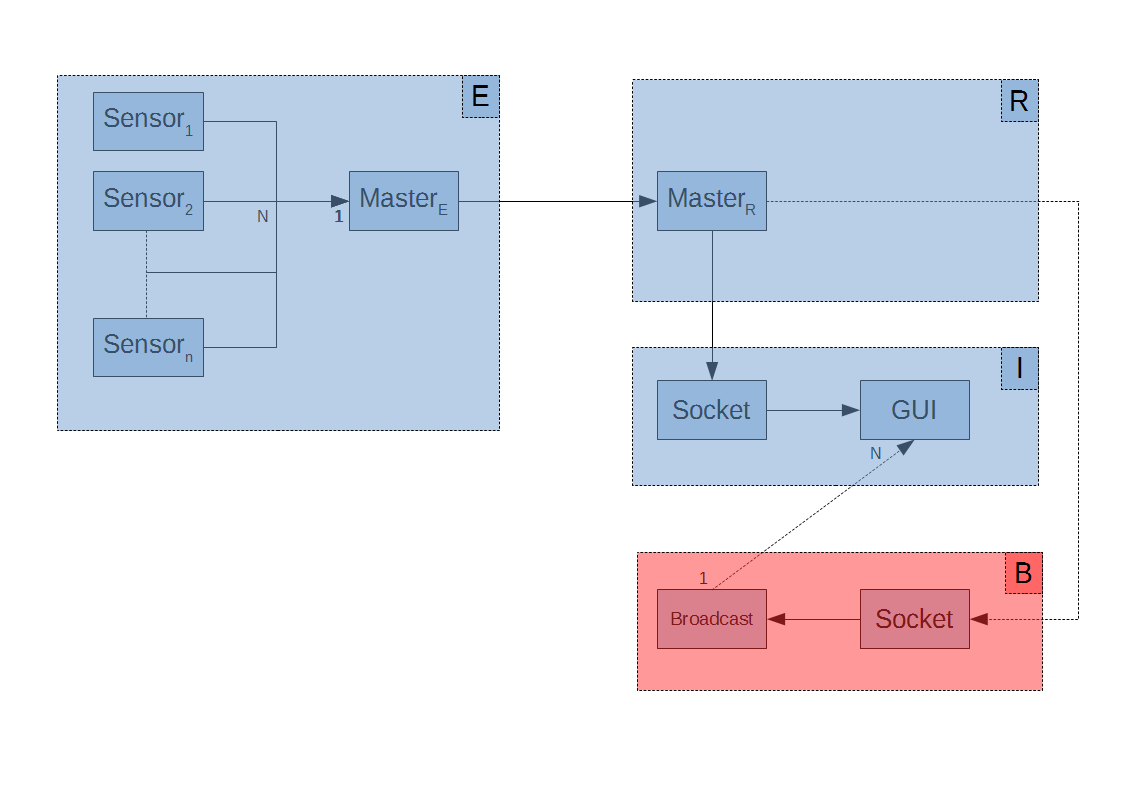
\includegraphics[width=\linewidth]{ERBI-Model-EtherCat}
		\subcaption{EtherCAT variation}
		\label{fig:catmodel}
	\end{minipage}
	\rulesep
	\begin{minipage}{.49\textwidth}
		\centering
		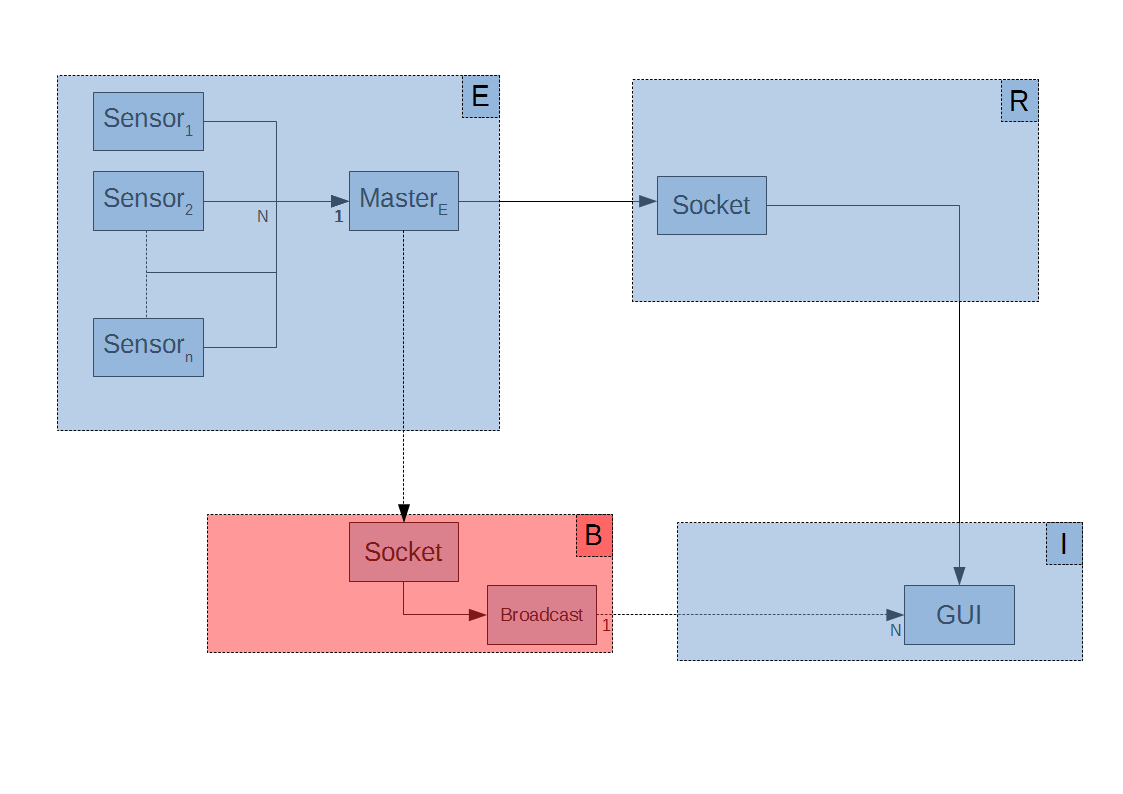
\includegraphics[width=\linewidth]{ERBI-Model-TCP}
		\subcaption{Ethernet variation}
		\label{fig:netmodel}
	\end{minipage}
	\caption{The variations of the original model}
	\label{fig:firstmodel}
\end{figure}

\subsection{Improved model}
Add a Raspberry Pi
\subsubsection{Plan A}
The Matlab GUI Model
UDP Send: \cite{web:UDPSend}
\subsubsection{Plan B}
The Standalone Model
\subsubsection{Plan C}
The Webservice Model

\subsection{Data Packaging}
\begin{itemize}
	\item Two custom blocks in Matlab
	\item State Table
	\item Update rate 50 Hz
\end{itemize}